\chapter{Pre and post processing work preparation}
\label{Chapter2}

\section{Introduction}

To complete

\section{Tools used during the test}

\subsection{MMCG test piece}

The MMCG test piece was developed by \cite{MoutouPitti2008}. However, the specimens tested at the University of Lisbon are not of the same dimensions. After carefully measuring the specimens, it turns out that they have the same dimensions as the specimens studied by Odounga. Below are the dimensions of the specimens that will be tested figure \ref{fig:fig23}:


\begin{figure}[htp]
	\centering
	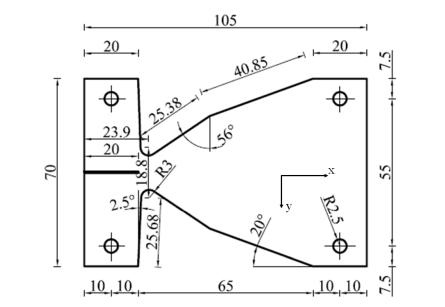
\includegraphics[width=8cm]{fig23}
	\caption{Dimensions of the tested MMCG specimen}
	\label{fig:fig23}
\end{figure}

\subsection{Arcan model and final grips}

To perform the tests, a steel Arcan system must be designed. It is made of high tensile steel (HLE). Indeed, this part allows to connect the 2MCG wood specimen to the press. In order to create this grip we must first take into account the dimensions of the 2MCG specimen available in Nova school described in figure \ref{fig:fig24}. The shape of the Arcan system must also allow a good visibility on the propagation of the crack. Figure 21 shows the Arcan device that we will use, which was inspired from the thesis of \cite{Odounga2018phd}.


\begin{figure}[htp]
	\centering
	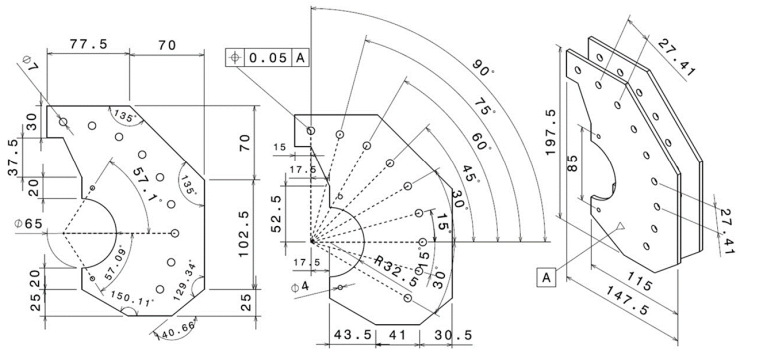
\includegraphics[width=15cm]{fig24}
	\caption{Size of the Arcan fastening system \cite{Odounga2018phd}}
	\label{fig:fig24}
\end{figure}

The fixing holes for the wooden specimens have a diameter $\Phi= 5 mm$, and the loading holes have a diameter $\Phi = 7 mm$. These fixing holes were drilled in order to be able to load the specimen with different angular values of the angle in relation to the vertical direction in order to activate different failure modes depending on the load angle. To connect the Arcan system to the press, a piece had to be created, as shown in figure \ref{fig:fig25}.


\begin{figure}[htp]
	\centering
	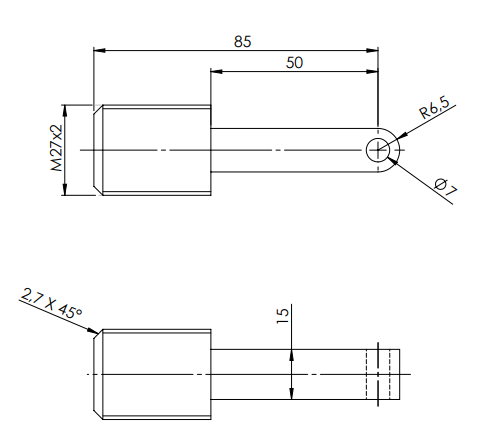
\includegraphics[width=6cm]{fig25}
	\caption{Bolt for connecting the press and the Arcan System}
	\label{fig:fig25}
\end{figure}

This part has a hole of the same size as the holes of the Arcan system in order to connect them. Moreover the head of the connector is 27mm in diameter and the thread has a 2mm pitch to connect to the press. Before sending the technical drawings to a company, a 3D printer was used to verify that the system worked properly. It was then necessary to draw the assembly on solidworks in order to print the assembly and send the technical drawings. Figure \ref{fig:fig26} shows the assembled device in Solidworks.


\begin{figure}[htp]
	\centering
	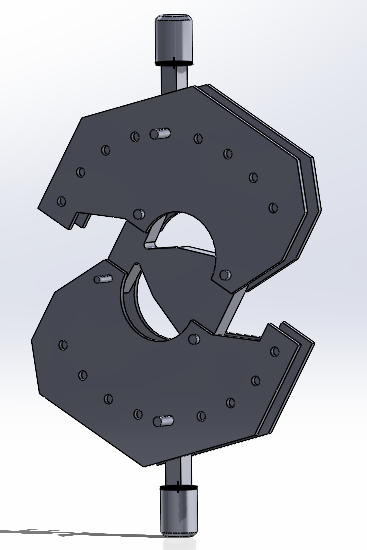
\includegraphics[width=5cm]{fig26}
	\caption{Assembled device in Solidworks}
	\label{fig:fig26}
\end{figure}

It has been shown in previous work such as \cite{Odounga2018phd} that one of the main problems with the MMCG specimen is the small distance between the holes and specimen extremities. This implies several cracks in the heel between the hole and the extremity of the sample which prevents observation and analysis of the fracture. One solution proposed by Odounga is the use of washers which could be glued or to strength screw the nut. Indeed, by applying compressive stress on each side of the sample, it reduces the stress applied on the holes and distributes the load in a wider area.

\subsection{Hydraulic press used}

To determine experimental parameters like the load speed or the frequency of the camera recording, it was important to read previous works on the subject and determine which engines will be used to proceed the experiments. The press used for the tests is a Landmark Servohydraulic Test Systems model 661.21B-03  from MTS. It is capable of exerting a maximal applied load of 10 metric to N (figure \ref{fig:fig27}).
In the work of \cite{Ostapska2021} the load speed recommended was about $0.1\ mm\ {min}^{-1}$ and the record was made at a frequency of 5 Hz, so 5 images per seconds. In the work of Mambili the record was made at a frequency of 10 Hz and the load speed was about 0.3 mm/s with a pre-load of 100N. It should be remembered that this press is also chosen because of its ability to load the specimens with a constant time displacement. Indeed, it was explained that this work will use the complacency method to compare the results.

As explained \cite{MALFAIT2021}  this MTS Hydraulic Press works with a cooler fluid. Indeed, a tank full of fluid mixed to water and a cooler system send this fluid mix to the press as visible on 23. Then, a hydraulic supply from MTS sends this liquid to the press itself. It is the model 506.02 serie 22 coupled with the Vickers DG4V-3-2A. Then the pressure is created thanks to the Hydraulic Service Manifold part from MTS company, model 234.11. Finally, a servo valve MOOG A076-263c increase the pressure to allow the hydraulic press operation. It is a high performance valve which drives a dry torque motor. Then a MTS load cell (661-21B-03) allows to follow the displacement of the hydraulic press.


\begin{figure}[htp]
	\centering
	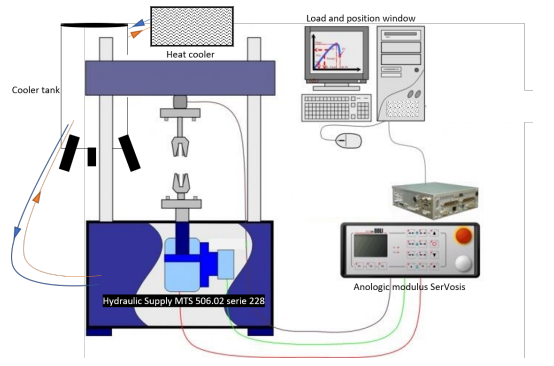
\includegraphics[width=10cm]{fig27}
	\caption{Hydraulic Press components allowing it use}
	\label{fig:fig27}
\end{figure}

To avoid displacement of the specimens, a preload is applied to the wood specimen. In the tests performed by \cite{MALFAIT2021} this preload was ignored to avoid negative loading values. An offset was applied to the P-$\delta$ to avoid these negative values which do not make sense. By ignoring this first loading, all results are truncated and the impacts on other parameters such as the energy release rate is disastrous. 
To remedy this problem, it is necessary to examine the load of the hydraulic press before it is used. This value, even if it is negative, will be subtracted from all the others, which will give the preload. Another solution is to continue testing, even after the propagation in the ZOI has ended. Indeed, the value of the load at the end of the test, on a collapsed specimen, will be equal to zero, even if the zero value is negative.

\section{Research and understanding of the parameters of the DIC method}

\subsection{Characteristic of the Wood used}

In this section, the values of the mechanical characteristics (moduli of elasticity, compliances and shear coefficients) are given. As no characterization tests were carried out in this study, the data from the literature are used here, following the document created by \cite{GuitardandElAmri1987}. These values which are the shearing $G_{ij}$ and longitudinal modulus $E_i$ , the Poisson’s coefficient $\nu_{ij}$ and $\rho$ change for each species. Moreover, these values can evolve due to temperature and relative humidity. By knowing the temperature, the relative humidity and the volume weight of a specimen, it is possible to obtain the characteristics wanted. Table \ref{fig:fig28} and \ref{fig:fig29} give us the characteristics for the Pinus Sp Pine at 9.7$\%$ humidity:


\begin{table}[htp]
	\centering
	
\includegraphics[width=10cm]{fig28}
	\label{fig:fig28}
\end{table}


\begin{table}[htp]
	\centering
	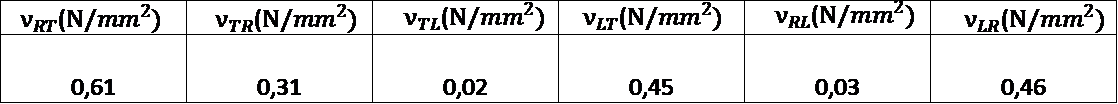
\includegraphics[width=10cm]{fig29}
	\caption{Characteristic of the Pinus Sp Pine}
	\label{fig:fig29}
\end{table}

\subsection{Preparation of the DIC method}

It is possible to process the images with different software. This image processing will allow to obtain the maps of deformations and displacements. For this work will be used MatchID and python. In our case, the quantity of interest is the crack length a as a function of the applied force F. The field of view ( FOV), the position envelope for hardware and if the test is a 2D-DIC or a stereo DIC are parameters to take into account. In our case, a 2D-DIC is suitable because the test piece is assumed to be planar and perpendicular to the camera optical axis. The DIC pattern is one important parameter. All the specimens are painted to obtain a speckle pattern suitable for image correlation. A thin layer of white paint is firstly added using a mate spray, followed by a diffuse distribution of black paint to create a unique local pattern across the ZOI at the crack tip.

Before starting the test, some parameters must be set on MatchID.grab. It is possible to vary parameters such as the exposure time. The speckle pattern is an image composed of black and white dots. By varying the exposure time, the speckle pattern will have a greater or lesser range of gray (from 0 to 255). On the other hand, a longer exposure time will result in color saturation. Then, it is important to adjust the quality of the speckle using two parameters, the focus and the aperture. With some cameras, it is sometimes impossible to adjust the focus. It is therefore necessary to play with the distance camera-specimen. After adjusting these 3 parameters, the calibration can begin. Its goal is to establish the image scale. It is necessary to take at least 50 images of a calibration sheet given by MatchID while making translations and rotations of this sheet.
After saving the calibration data, it is no longer possible to change these parameters. This calibration will be used for the tests.

\subsection{MatchID}

After calibration and recording of the tests, the datas must be processed. Several steps are necessary:

\begin{itemize}
	\item Choose a reference image that corresponds to the first image of the test 
	\item Select multiple deformed images
	\item Define the zone of interest (ZOI) in which the crack propagates
	\item Define the analysis parameters of the ZOI
	\item Start the DIC analysis
	\item Exploit the results
\end{itemize}

Despite the progress and increasing use of DIC, the technique is still not standardized. It is emphasized that extrinsic and intrinsic DIC setup parameters, such as subset size, subset step, strain gauge window, shape functions, or correlation criterion, can have a considerable influence on the calculated strain fields, producing spatial resolution and resolution values that can differ by at least an order of magnitude \cite{DICguide2018}. The next paragraph will try to explain some of them. 

\begin{itemize}
	\item The \textbf{correlation criterion} defines the matching criterion that will be adopted in order to determine the optimum corresponding point. \cite{MALFAIT2021}  used the criterion ZNSSD. It is a least-square-based correlation criterion which is less sensitive to both image contrast reduction and light intensity shifting between images. It's a robust correlation criterion which can be used with confidence. 
	\item There are 5 \textbf{subset shape function} which allow or not the subset certain constraints as the fact of translating, deforming, to shear etc.. Depending on the local deformation or strain gradients of the problem under analysis, affine, irregular and quadratic shape functions can be selected by the user in the DIC method \cite{PereiraandXavier2018}. 
	\item The \textbf{subset size} is the length of the subset in the reference image and it must contain at least 3 speckles. As an indication, larger subsets improve resolution but decrease spatial resolution. This means that in a conventional mechanical tensile test with a uniform, uniaxial stress state in the central region of the specimen, large subsets can be selected to improve the accuracy of the measurements.
	\item The \textbf{step size} is the spacing of pixel grid points at which the subset displacements are calculated. It controls the density of points at which DIC data is computed and, to some extent, influences the spatial resolution of the measurements. Typically, a step size of one-third to one-half of the subset size is recommended, so that neighboring subsets partially overlap, though this value can vary widely depending on specific applications. Additionally, a small step size may be required to capture the peak position of a Quantity Of Interest (QOI) (without interpolation) if it varies quickly across the ZOI and if the QOI varies slowly across the ZOI, then a large step size can be used. 
	\item The \textbf{strain window} is the local region of the ZOI of the image, containing a finite number of data points, that is used to calculate strain. Parameters such as the subset step and the strain window will define a strain spatial resolution and virtual strain gauge (VSG). 
	\item \textbf{VSG} is the local region of the image that affects the strain value at a specific location. The three dominant variables that affect the VSG size are the subset size, step size, and strain window. If the maximum strain amplitude converges with further decreases of the VSG, then the actual maximum strain amplitude has been captured. Any VSG that is larger than the largest VSG that results in the converged actual maximum strain amplitude will underestimate the actual strain amplitude, and introduce bias into the measured strain results. If the smallest VSG allowed by the software is not sufficient, the test could be repeated with a smaller FOV. The final decision as to which size VSG to use is a matter of judgment. If capturing the highest strain gradient is essential for DIC analysis, a small VSG may be the best choice, even if noise is important. Conversely, if there are no high strain gradients it may be preferable to choose a larger VSG to reduce uncertainties.
\end{itemize}

In order to determine the correct settings MatchID has a tool called Performance Analysis. With this tool, it’s possible to define a range of options to be applied in a design of experiments study. It is thus possible to vary parameters such as subset size, step size, strain window and so on. After running the performance analysis, select the parameters which work best(video 20). 
For the case of a uniaxial tensile test on a pre-cracked specimen by default the indicated zone of interest contains one initial subset but the ZOI is not well defined. In order to define well the ZOI it must be added an extra seed point in the ZOI but above the initial crack. After this, start the DIC analysis and exploit the results. To exploit the results in MatchID, it is possible to import data. In this case, import the data on the force applied throughout the test in order to plot the force as a function of the displacements for example (video 11).



\section{Python}

Python is a computer programming language often used to create websites and software, automate tasks and perform data analysis. It is a versatile language, which means that it can be used to create a variety of different programs and is not specialized for specific problems. This versatility, along with its beginner-friendliness, has made it one of the most widely used programming languages today.

A second data processing is necessary to obtain the position of the crack front and the displacements. This will allow later to plot the force as a function of the crack opening or as a function of the crack length. This will also allow to plot the energy release rate G as a function of the crack length a. Below are described two methods:

\subsection{Method 1}

\textbf{Mapping function and mapping mask}

The method used is based on the variation of the relative position between adjacent subsets which gives an estimate of the damage occurrence \cite{Xavieretal2014}. To begin with, a matching function A(x,y) is determined based on the norm of the relative position vectors as follows:

\begin{equation}
	A(x,y)=max(\lVert u_i-u_k\rVert;\lVert u_j-u_l\rVert)
\end{equation}

where $u_{i,j,k,l}$ represent the displacement vector of four adjacent subsets. A mapping mask is then defined assuming threshold segmentation according to the following inequalities.

\begin{equation}
	M(x,y)=
	\begin{cases}
		1 \text{ if } A(x,y) \geq \alpha \overline{A} \\
		0 \text{ if } A(x,y)< \alpha \overline{A}\\
		-1 \text{ if } A(x,y)= no data 
	\end{cases}
\end{equation}

The matrix M represents, for a given step, the length of the crack by having a larger value in the crack area. If the user looks too close, the noise of the values will prevent a good analysis, but looking too high on the matrix, the crack length value will not be accurate. To move around and get an accurate idea of how the user can look at the M matrix, it is important to use $\alpha$. The alpha parameter is like a cutting tool that allows one to get as close to the noise as possible without problems. Thus, when a subset is outside this region, it will be considered as zero. Then, subsets that are placed in the crack, or somewhere where there is a defect or missing information as in the crack, the subset will be defined with a value equal to -1. Then, for all the subsets around the crack, which have a real interest in the study, they will take the value equal to 1. Using this sub-step matrix, now composed of -1, 0, 1, it is possible to plot the whole matrix in shades of gray, and to have an overview of the crack development.

\textbf{$\alpha$ parameter}

The parameter $\alpha$ is selected as the lowest integer satisfying the inequality:

\begin{equation}
	a(\alpha)-a_0 < f_s, \alpha \in \mathbb{N}
\end{equation}

where fs is the spatial resolution associated to DIC measurements.

\textbf{Crack opening displacement}

To obtain CTOD, it is important to pay attention to the choice a0. Indeed, the chosen subset will be determinant. By considering the image as a matrix composed of subsets, the chosen subset is a position given by its m rows and n columns. Looking at the subset from top to bottom allows one to follow the displacement of the crack tip and measure it. The point is to determine which pair of subsets is the best which means being closer or less close to the crack. If one is too close to the crack there will be no information and if one is too far away the measurement will be less accurate. By looking at these displacements, it is possible to obtain the value of the crack opening at each step.

\textbf{Crack length}

A final part of the code allows us to obtain a(t) as a function of alpha. This is done by focusing on the ZOI and the number of subsets that compose it. Through the matrix composed by each subset, the displacement field can be observed. It is obtained by calculating the distance between the center of a subset and its displacement from one image to another, as described in the literature review. To simplify the code, this calculation is not performed on each subset but only on the four corners. By calculating the distance between the opposite corners, the maximum displacement in x and the displacement in y are introduced in a last matrix.

\subsection{Method 2}

\textbf{Crack opening displacement (COD) or Virtual displacement}

From the reference and current positions of the DIC calculation points, the Euclidean distance between each pair of points can be measured and the COD can be determined as follow:

\begin{equation}
	VD(k,i_n)=\sqrt{(x_{11bk}-x_{11tk})^2 + (x_{22bk}-x_{22tk})^2}_{i_n} - VD(k,i_0)
\end{equation}

where the indices t and b refer to the DIC data points located at the top and bottom of the crack path, k is the index of the DIC point, in is the image captured at time n, VD(k, i0) is the initial Euclidean distance between the computational points of the top and bottom reference DIC subset obtained from image i0, and $x_{11}$ and $x_{22}$ are their coordinates in the image plane.

\textbf{$\alpha$ and $\beta$ parameters}

The first step towards detecting the crack tip is to take the average value of VD:

\begin{equation}
	\overline{VD}(i_n)=\frac{1}{k} \sum_{k=1}^{k}VD(k,i_n)
\end{equation}

The threshold value need to be adjusted with 2 parameters $\alpha$ and $\beta$ which are defined below:

\begin{equation}
	\alpha=\frac{w_0 - w_f}{i_0 - i_f}  and \beta=w_0- \alpha i_0
\end{equation}

where $w_0$ and $w_f$ can be expressed as a factor used to adjust the model to the initial ($p_0$) and final ($p_f$) crack tip positions, respectively, along $x_{11}$ axis. A virtual manual detection is performed to initialize $p_0$ and $p_f$.

Therefore, the adjusted threshold line-cut (VDth) is given by:

\begin{equation}
	VD_{th}(i_n)=\overline{VD}(i_n)(\alpha i_n +\beta)
\end{equation}

The intersection between each $VD_{th}(i_n)$ and the corresponding $VD(k, i_n)$ curve at time n represents the $x_{11}$ position of the crack tip, denoted by ($p_n$).
It is therefore possible to calculate the growth of the crack at instant n:

\begin{equation}
	da_n=p_n-p_0
\end{equation}

\subsection{Energy restitution rate}

After using one of the two previous methods, we can calculate the energy restitution rate in mode 1 and in mixed mode.

For mode 1, the formula is the one explained in chapter 1:

\begin{equation}
	G_c=\frac{{F_{ci}}^2}{2b}\ \frac{\partial C}{\partial a}
\end{equation}

For mixed mode, the formula becomes:

\begin{equation}
	\begin{cases}
		G_I=\frac{{F_{cx}}^2}{2b}\ \frac{\partial C}{\partial a} \\
		G_{II}=\frac{{F_{cy}}^2}{2b}\ \frac{\partial C}{\partial a}\\ 
	\end{cases}
\end{equation}

In mixed mode the camera will have the same inclination as the specimen. The crack opening values will therefore be projected directly along the x and y axes. The force is projected along the x and y axes, so we have:

\begin{equation}
	\begin{cases}
		F_{cy}=F \sin(\alpha) \\
		F_{cx}=F \cos(\alpha) \\ 
	\end{cases}
\end{equation}

\section{Specimen preparation}

\subsection{Notch and precrack}

Notches were created in each specimen. A precrack is made by a cutter into the notch. The interest is to initiate a straight crack, thanks to this first one. The notch width is around 1.5mm, done by a straight electrical saw. The cutter allow to go deeper and create a precrack with a shape allowing the propagation of the crack. The precrack must be done at the center of the sample heel. Indeed, even a little eccentricity could cause a deviation of the crack and prevent a good study of the propagation. The specimen was designed with an initial crack noted $a_i$ of length  $a_i=22mm$. The total crack length is equal to: $a=a_i+\Delta a$.


\section{Conclusion}

To complete


